\documentclass[aspectratio=169,10pt]{beamer}
\usepackage[T1]{fontenc}
\usepackage{lmodern}
\usepackage{amsmath,amssymb}
\usepackage{booktabs}
\usepackage{tikz}
\usepackage{tabularx}
\usetikzlibrary{arrows.meta,positioning,fit}
\usepackage{xcolor}
\usepackage{hyperref}
\hypersetup{colorlinks=true,urlcolor=accent}

\definecolor{accent}{HTML}{0B5563}
\definecolor{accent2}{HTML}{0F766E}
\definecolor{warn}{HTML}{B45309}
\definecolor{muted}{HTML}{4B5563}
\setbeamercolor{frametitle}{bg=accent,fg=white}
\setbeamercolor{title}{fg=accent}
\setbeamercolor{structure}{fg=accent}
\setbeamercolor{normal text}{fg=black!88}
\setbeamercolor{block title}{bg=accent!12,fg=accent}
\setbeamercolor{block body}{bg=accent!4}
\setbeamertemplate{navigation symbols}{}
\setbeamertemplate{itemize items}[circle]
\setbeamertemplate{footline}{%
  \hfill{\color{muted}\scriptsize wvyern \quad\insertframenumber\,/\,\inserttotalframenumber}\hspace{4mm}\vspace{2mm}}
\setbeamerfont{frametitle}{series=\bfseries,size=\large}
\setbeamerfont{title}{series=\bfseries,size=\LARGE}
\newcommand{\code}[1]{\texttt{#1}}
\newcommand{\hl}[1]{\textcolor{accent}{\textbf{#1}}}
\newcommand{\warnt}[1]{\textcolor{warn}{\textbf{#1}}}

\begin{document}

% ---------------------------------------------------------------- 1
\begin{frame}[plain]
\vspace{10mm}
{\usebeamerfont{title}Clinical Term Mapping\par}
\vspace{2mm}
{\large Entity + note context $\rightarrow$ ICD-10-CM code \& SNOMED CT concept\par}
\vspace{7mm}
{\color{muted}wvyern \;|\; Final approach and demo\par}
\vspace{6mm}
\begin{columns}[T]
\begin{column}{0.48\textwidth}
\begin{block}{Dev (780 questions)}
ICD \hl{0.573} \quad SNOMED \hl{0.667}\\[1pt]
{\small shortlist recall 0.82 / 0.89}
\end{block}
\end{column}
\begin{column}{0.48\textwidth}
\begin{block}{Test (1{,}025 questions)}
ICD \hl{0.564} \quad SNOMED \hl{0.612}\\[1pt]
{\small overall 0.590; headline = lower system}
\end{block}
\end{column}
\end{columns}
\vspace{4mm}
{\small\color{muted}Two stages: judge-ranked shortlist $\rightarrow$ calibrated decision model, ensembled over option orders.}
\end{frame}

% ---------------------------------------------------------------- 2
\begin{frame}{Problem, data, and what makes it hard}
\begin{columns}[T]
\begin{column}{0.52\textwidth}
\textbf{Task}\\[1pt]
One entity + its note context $\rightarrow$ exactly one ICD-10-CM and one SNOMED CT id.

\vspace{3mm}
\textbf{Data}\\
2{,}882 entity/chunk pairs; leak-free splits\\[1pt]
{\small train 1{,}873 \;\textbar\; dev 432 \;\textbar\; test 577}

\vspace{3mm}
\textbf{Metric}\\
Exact match per system; \hl{headline = lower of the two}.
\end{column}
\begin{column}{0.44\textwidth}
\textbf{Why it is hard}
\begin{itemize}\setlength\itemsep{1.5pt}
\item \textbf{Long tail:} 32\% of dev ICD and 64\% of dev SNOMED golds never appear in train.
\item \textbf{Conventions:} gold \code{E78.0} vs.\ billable child \code{E78.00}.
\item \textbf{Noise:} abbreviations (\emph{lee}), OCR artifacts (\emph{\o{} tremor}).
\item \textbf{Near-duplicate codes:} right concept, wrong specificity.
\end{itemize}
\end{column}
\end{columns}
\end{frame}

% ---------------------------------------------------------------- 3
\begin{frame}{Architecture: retrieval, then a calibrated decision}
\centering
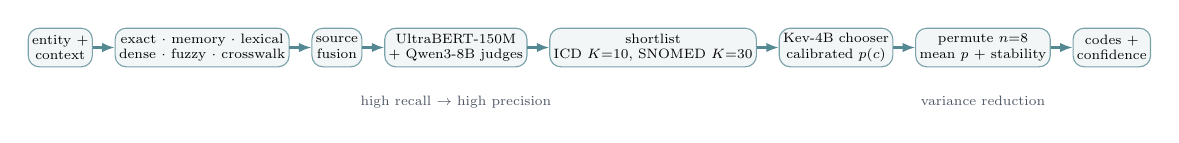
\begin{tikzpicture}[scale=0.7, transform shape,
  box/.style={draw=accent!55, fill=accent!5, rounded corners, align=center, font=\scriptsize, inner sep=2pt, minimum height=7mm},
  arr/.style={-{Latex[length=1.6mm]}, thick, draw=accent!70},
  node distance=3mm and 4mm]
\node[box] (in) {entity +\\ context};
\node[box, right=of in] (src) {exact $\cdot$ memory $\cdot$ lexical\\dense $\cdot$ fuzzy $\cdot$ crosswalk};
\node[box, right=of src] (fus) {source\\fusion};
\node[box, right=of fus] (jud) {UltraBERT-150M\\+ Qwen3-8B judges};
\node[box, right=of jud] (sl) {shortlist\\ICD $K{=}10$, SNOMED $K{=}30$};
\node[box, right=of sl] (kev) {Kev-4B chooser\\calibrated $p(c)$};
\node[box, right=of kev] (ens) {permute $n{=}8$\\mean $p$ + stability};
\node[box, right=of ens] (out) {codes +\\ confidence};
\foreach \a/\b in {in/src, src/fus, fus/jud, jud/sl, sl/kev, kev/ens, ens/out} \draw[arr] (\a) -- (\b);
\node[font=\scriptsize\color{muted}, below=4mm of jud] {high recall $\rightarrow$ high precision};
\node[font=\scriptsize\color{muted}, below=4mm of ens] {variance reduction};
\end{tikzpicture}

\vspace{5mm}
\begin{columns}[T]
\begin{column}{0.48\textwidth}
\begin{block}{Stage 1 --- shortlist}
7 candidate sources + 3 dense encoders; two judges rank candidates; keep $K$ small to avoid near-gold decoys.
\end{block}
\end{column}
\begin{column}{0.48\textwidth}
\begin{block}{Stage 2 --- chooser}
Small decision model returns probabilities, not text; permutation ensemble removes order sensitivity.
\end{block}
\end{column}
\end{columns}
\end{frame}

% ---------------------------------------------------------------- 4
\begin{frame}{Stage 1: candidate pool $\rightarrow$ shortlist}
\begin{columns}[T]
\begin{column}{0.50\textwidth}
\textbf{Candidates}\\
exact $\cdot$ memory $\cdot$ lexical $\cdot$ dense $\cdot$ fuzzy $\cdot$ crosswalk $\cdot$ char-ngram\\[1pt]
{\small dense pool: gte-base + BioLORD + UltraBERT-Embed (weight 0.84)}

\vspace{3mm}
\textbf{Judges}\\
UltraBERT-150M pairwise, fine-tuned on 60.6k pairs vs.\ 20 hard negatives\\
Qwen3-Reranker-8B (zero-shot)\\
blend: $j=0.5\,z_u+0.5\,z_q$

\vspace{3mm}
\textbf{Shortlist}\\
rank by $\;w\,\hat j+(1-w)\,\hat f$, top-$K$
\end{column}
\begin{column}{0.46\textwidth}
\begin{block}{Configuration \& recall}
\small
\begin{tabular}{@{}lccc@{}}
\toprule
System & Judge & $w$ & $K$\\
\midrule
ICD & UltraBERT & 0.2 & 10\\
SNOMED & combined & 0.6 & 30\\
\bottomrule
\end{tabular}\\[2mm]
dev recall \hl{0.818} / \hl{0.887}\\
test recall (config B) 0.838 / 0.874
\end{block}
\vspace{2mm}
{\small\color{muted}Larger $K$ raises recall but seeds decoys: measured on dev, it \emph{lowers} accuracy.}
\end{column}
\end{columns}
\end{frame}

% ---------------------------------------------------------------- 5
\begin{frame}{Stage 2: calibrated chooser + permutation ensemble}
\begin{columns}[T]
\begin{column}{0.50\textwidth}
\textbf{Kev-4B} (Qwen3.5-4B-Base + LoRA + pointer head)
\begin{itemize}\setlength\itemsep{1pt}
\item Prefill-only: returns a probability for every candidate. No generation.
\item Questions isolated; checkpoint ships a fitted temperature.
\item Trained on 1{,}776 examples built with the \emph{inference} recipe; 2 epochs, 44 min.
\end{itemize}
\vspace{2mm}
\textbf{Why not a generative LLM?}\\
Qwen3.5-4B instruct replacement: \warnt{0.402 / 0.408}; it re-codes clinically and ignores dataset conventions.
\end{column}
\begin{column}{0.46\textwidth}
\begin{block}{Permutation ensemble}
\[
\bar p(c)=\frac{1}{n}\sum_{t=1}^{n} p_t(c \mid \pi_t)
\]
predict $\arg\max_c \bar p(c)$; record margin $\bar p_{(1)}-\bar p_{(2)}$ and stability.\\[2mm]
$n{=}8$ option orders (seeded).\\[2mm]
dev ICD \hl{0.548 $\rightarrow$ 0.573}\\
dev SNOMED \hl{0.647 $\rightarrow$ 0.667}
\end{block}
{\small\color{muted}Order alone can swing accuracy $\sim$1.4 pts.}
\end{column}
\end{columns}
\end{frame}

% ---------------------------------------------------------------- 6
\begin{frame}{Results}
\begin{columns}[T]
\begin{column}{0.55\textwidth}
\small
\begin{tabular}{@{}llrrr@{}}
\toprule
Split & Config & ICD & SNOMED & All\\
\midrule
dev & A, single & 0.548 & 0.647 & 0.598\\
dev & A, perm.\ $n{=}8$ & \hl{0.573} & \hl{0.667} & \hl{0.620}\\
test & A, single & 0.532 & 0.603 & 0.571\\
test & B, perm.\ $n{=}8$ & \hl{0.564} & \hl{0.612} & \hl{0.590}\\
\bottomrule
\end{tabular}\\[2mm]
{\footnotesize B = ICD shortlist widened to $K{=}20$ with the combined judge (test recall 71\%$\rightarrow$84\%).}
\end{column}
\begin{column}{0.42\textwidth}
\begin{block}{Diagnostics (test)}
\small
shortlist recall 0.838 / 0.874\\
acc$|$present 0.673 / 0.700\\
ICD 3-char partial credit \hl{0.748}\\
unseen-gold accuracy 0.507 / 0.564\\[1mm]
{\footnotesize unseen golds: 146 ICD / 319 SNOMED}
\end{block}
\end{column}
\end{columns}
\end{frame}

% ---------------------------------------------------------------- 7
\begin{frame}{Where it fails --- and the demo cases}
\begin{columns}[T]
\begin{column}{0.52\textwidth}
\footnotesize
\begin{tabularx}{\linewidth}{@{}lXl@{}}
\toprule
Entity & Failure mode & Pick / gold\\
\midrule
\emph{ich} & abbreviation & I61.9 / I61.9\\
\emph{lee} & abbrev.\ collision & \warnt{A57} / I89.0\\
\emph{\o{} tremor} & OCR artifact & R25.1 / R25.1\\
\emph{t2dm poorly controlled} & specificity & E11.65 / E11.65\\
\emph{hypercholesteremia} & convention & \warnt{E78.0} / E78.00\\
\emph{pulmonary nodule} & sibling near-miss & \warnt{R91.8} / R91.1\\
\bottomrule
\end{tabularx}
\vspace{2mm}

{\footnotesize demo: \texttt{python demo/inspect.py} shows top-3 probabilities, margin, stability.}
\end{column}
\begin{column}{0.44\textwidth}
\begin{block}{Coverage / abstention (test)}
\small
\begin{tabular}{@{}lcc@{}}
\toprule
coverage & ICD & SNOMED\\
\midrule
100\% & 0.564 & 0.612\\
70\% & 0.679 & 0.740\\
60\% & \hl{0.721} & \hl{0.770}\\
50\% & 0.761 & 0.809\\
\bottomrule
\end{tabular}\\[1mm]
{\footnotesize rank by ensemble margin}
\end{block}
\vspace{2mm}
{\small Error split: ICD 66 retrieval / 89 chooser; SNOMED 47 / 92.\\[1pt]
61 of 155 ICD errors are same-block siblings.}
\end{column}
\end{columns}
\end{frame}

% ---------------------------------------------------------------- 8
\begin{frame}{What did not work, and what is next}
\begin{columns}[T]
\begin{column}{0.52\textwidth}
\textbf{Measured and rejected}
\begin{itemize}\setlength\itemsep{1pt}
\item[$\times$] Larger $K$ on dev (0.521 / 0.548)
\item[$\times$] Alignment retrain on served shortlists (0.532 / 0.609)
\item[$\times$] Generative chooser (0.402 / 0.408)
\item[$\times$] Gemma-4 arbitration (harmful / neutral)
\item[$\times$] Imported fine-tuned SapBERT+CE ICD stack (0.556--0.588)
\item[$\times$] Longer criteria / full context / hierarchy-first (no change)
\end{itemize}
\end{column}
\begin{column}{0.44\textwidth}
\textbf{Next}
\begin{itemize}\setlength\itemsep{1pt}
\item[$\rightarrow$] Parent/child \emph{convention} tie-break learned from train labels
\item[$\rightarrow$] Evidence-aware arbitration only on low-margin rows
\item[$\rightarrow$] Kev-9B/27B (drop-in; blocked by shared GPUs)
\item[$\rightarrow$] ICD recall: sibling expansion + recall-oriented judge
\item[$\rightarrow$] Ship calibrated abstention (60\% at $\sim$0.72--0.77)
\end{itemize}
\end{column}
\end{columns}
\vspace{4mm}
\begin{block}{Artifacts}
\footnotesize
Repo \texttt{hilabs-submission} \;|\;
chooser \url{https://huggingface.co/d3let3/kev-4b-clinical-mapping} \;|\;
judge \url{https://huggingface.co/d3let3/ultrabert-clinical-judge}\\
Demo video: \texttt{TBD}
\end{block}
\end{frame}

\end{document}
